
\documentclass[12pt]{article}
%%%%%%%%%%%%%%%%%%%%%%%%%%%%%%%%%%%%%%%%%%%%%%%%%%%%%%%%%%%%%%%%%%%%%%%%%%%%%%%%%%%%%%%%%%%%%%%%%%%%%%%%%%%%%%%%%%%%%%%%%%%%%%%%%%%%%%%%%%%%%%%%%%%%%%%%%%%%%%%%%%%%%%%%%%%%%%%%%%%%%%%%%%%%%%%%%%%%%%%%%%%%%%%%%%%%%%%%%%%%%%%%%%%%%%%%%%%%%%%%%%%%%%%%%%%%
\usepackage{amsmath,amsthm}
\usepackage[latin1]{inputenc}
\usepackage[T1]{fontenc}
\usepackage{minionpro}
\usepackage{array,graphicx}

\setcounter{MaxMatrixCols}{10}
%TCIDATA{TCIstyle=LaTeX article (bright).cst}

%TCIDATA{OutputFilter=LATEX.DLL}
%TCIDATA{Version=5.00.0.2570}
%TCIDATA{<META NAME="SaveForMode" CONTENT="1">}
%TCIDATA{Created=Monday, January 29, 2007 11:45:31}
%TCIDATA{LastRevised=Friday, November 30, 2007 08:35:24}
%TCIDATA{<META NAME="GraphicsSave" CONTENT="32">}
%TCIDATA{<META NAME="DocumentShell" CONTENT="Exams and Syllabi\SW\Assignment">}
%TCIDATA{Language=American English}

\setlength{\topmargin}{-0.3in} \setlength{\textheight}{8.75in}
\setlength{\oddsidemargin}{0.0in} \setlength{\evensidemargin}{0.0in}
\setlength{\textwidth}{6.5in}
\def\labelenumi{\arabic{enumi}.}
\def\theenumi{\arabic{enumi}}
\def\labelenumii{(\alph{enumii})}
\def\theenumii{\alph{enumii}}
\def\p@enumii{\theenumi.}
\def\labelenumiii{\arabic{enumiii}.}
\def\theenumiii{\arabic{enumiii}}
\def\p@enumiii{(\theenumi)(\theenumii)}
\def\labelenumiv{\arabic{enumiv}.}
\def\theenumiv{\arabic{enumiv}}
\def\p@enumiv{\p@enumiii.\theenumiii}
\pagestyle{plain}
\pagestyle{plain} \setcounter{secnumdepth}{3}
\newcommand{\D}{\mathop{\mathrm{d\mathstrut}}\nolimits\!}
\newcommand{\dt}{\D t}
\newcommand{\dz}{\D z}
\newcommand{\E}{\mathop{\mathrm{E\mathstrut}}\nolimits}
\newcommand{\Var}{\mathop{\mathrm{Var\mathstrut}}\nolimits}
\newcommand{\sd}{\mathop{\mathrm{sd\mathstrut}}\nolimits}
\newcommand{\diag}{\mathop{\mathrm{diag\mathstrut}}\nolimits}
\newcommand{\Cov}{\mathop{\mathrm{Cov\mathstrut}}\nolimits}
\newcommand{\Corr}{\mathop{\mathrm{Corr\mathstrut}}\nolimits}
\newtheorem{definition}{Definition}
\newtheorem{proposition}{Proposition}
\newtheorem{conjecture}{Conjecture}
\newtheorem{moment}{Empirical regularity}
\newtheorem{insight}{Qualitative prediction}
%\input{tcilatex}

\begin{document}

\title{A Spatial Explanation for the Balassa--Samuelson Effect\thanks{\textsc{Preliminary and incomplete. Please do not circulate.}}}
\author{P\'eter Kar\'adi\thanks{New York University. E-mail: peter.karadi@nyu.edu}~ and Mikl\'os Koren\thanks{Princeton University. E-mail: mkoren@princeton.edu.}}
\maketitle

\begin{abstract}
We propose a model of urbanization and development to explain why the price level is higher in rich countries. There are two sectors: manufacturing, which is freely tradable, and non-tradable services, which have to locate near customers in big cities. As countries develop, total factor productivity increases simultaneously in both sectors. However, because services compete with the urban population for scarce land, labor productivity will grow slower in services than in manufacturing. Services become more expensive, and the aggregate price level becomes higher. The model hence provides a theoretical foundation for the Balassa--Samuelson assumption that productivity growth is slower in the non-tradable sector than in the tradable sector. The key implications of the model are borne out in the data: while the positive correlation between income and the price level is very strong among countries where land is scarce (densely populated, highly urban countries), there is virtually no such correlation among rural countries.
\end{abstract}

\section{Introduction}
Rich countries are more expensive than poor ones. Figure \ref{fig:penn_joint} shows
the strong correlation between aggregate price level and (PPP-adjusted) GDP per capita for 188 Penn-World-Table countries in 2000. Balassa (1964) and Samuelson
(1964) suggested a simple and powerful explanation based on the
observation that productivity growth of tradables, such as manufacturing,
tends to be faster than productivity growth of non-tradables, such as
services. Assuming that labor is perfectly mobile across sectors,
firms need to pay the same wage in both sectors in equilibrium, and
these wages are pinned down by the international price of the
tradable good and the productivity in the tradable sector.
Relatively lower non-tradable sector productivity, thereby, will
imply higher non-tradable prices. Empirical observations support the
major propositions of the model about the importance of the
non-tradable sector as well as the development of the relative
productivities and their effects on the relative prices (see e.g.
Obstfeld-Rogoff, 1996)\footnote{Hsieh and Klenow (1997) recently
argued that low PPP investment rates in poor countries come from
their low relative productivity in producing investment and tradable
goods relative to non-tradable consumption services.} Though
empirical results are also consistent with the assumption that total factor
productivity growth does tend to favor the tradable sector, the
theory falls short of providing an explanation for it.

Rich cities are more expensive than poor ones. According to \texttt{bestplaces.net}, the overall cost of living is 54 percent higher in Boston, MA than in Milwaukee, WI. The two cities are of similar size (close to 600,000 people), but the per capita income in Boston (\$28,000) is about 56 percent higher than that in Milwaukee (\$18,000). Similarly to the price differences across countries, the biggest price differences are in nontradable sectors. Healthcare is 33 percent more expensive in Boston, whereas housing is about 200 percent more expensive.\footnote{All data retrieved from \texttt{http://bestplaces.net} on January 30, 2008.} While the Balassa--Samuelson explanation has the potential to explain price differences across cities, some simple demand considerations also jump to mind. Demand for services is higher in high-income cities, while supply is limited, which drives up service prices. A scarce factor in cities that may limit the supply of services is land.\footnote{Tang (2007) offers an income-based explanation for the positive correlation between price level and GDP per capita. He does not focus on cities and the spatial distribution of economic activity, however.}

We propose a model of development and urbanization that reconciles these two facts and connects these two types of explanations. There are two sectors: manufacturing, which is freely tradable, and non-tradable services, which have to locate near customers in big cities. As countries develop, total factor productivity increases simultaneously in both sectors. However, because services compete with the urban population for scarce land, labor productivity will grow slower in services than in manufacturing. Services become more expensive, and the aggregate price level becomes higher with development.

Our model rests on three key observations.

First, land is scarcer than one might first think. The overall population density of the earth is rather low, 43 people per square kilometer.  However, population is very clustered, so the average person lives in an area with a population density of 5,700 people per square kilometer.\footnote{We used high-resolution population density data from LandScan to calculate, for the average person on earth, the number of people living within the same 30 arc second by 30 arc second area. (This is basically a population-weighted population density.) } A related observation is that in 2005, around 50 percent of the world population lived in cities.\footnote{World Development Indicators.} This suggests that the scarcity of land, which has the potential to explain price differences across cities, can also be partly responsible for price differences across countries.

Second, whether a good is tradable or not has implications not only for cross-country trade but also for within-country trade, and hence the location of production within the country. Arguably, there are many technological differences between tradable sectors such as manufacturing, and non-tradable sectors such as services. The fundamental difference, however, is that non-tradable goods or services have to be produced at the location of their consumption, whereas tradable goods and services can be produced far away from consumers, where land prices may be cheaper. Figure \ref{fig:ntcounties} shows a map of U.S.~counties, displaying the \emph{share} of employment in non-tradable sectors. Darker colors represent a higher share in non-tradable sectors. We see that non-tradable sectors locate closer to population centers than tradable sectors.\footnote{This is confirmed more formally in Section \ref{empirics}.} The implication of this observation is that non-tradable prices are more sensitive to the price of land than tradable prices.

\begin{figure}[h!]
%  \vspace*{-7em}
\centering
  % Requires \usepackage{graphicx}
  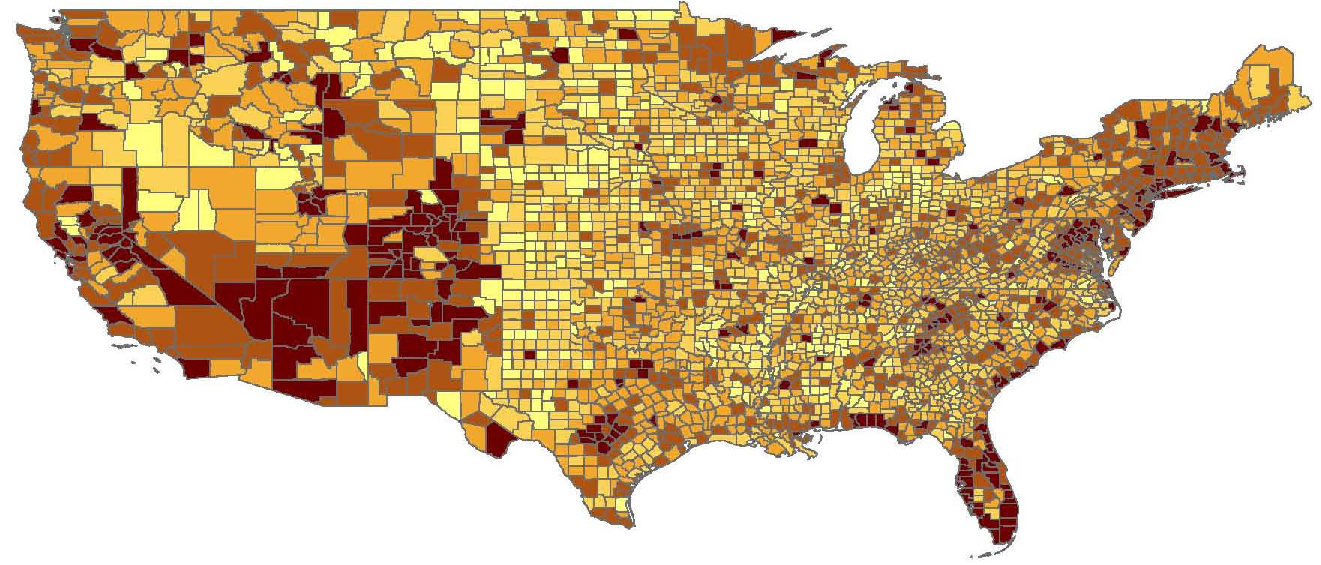
\includegraphics[width=0.7\linewidth]{figures/ntcounties}
  \vspace*{-1em}
  \caption{The share of non-traded employment in U.S.~counties}\label{fig:ntcounties}
  {\small\emph{Source}: 2000 U.S.~Census, Summary File 3.}
\end{figure}

Third, productivity growth in the housing sector is limited by the scarcity of land. Increased productivity in construction can lead to taller and higher-quality buildings, but they cannot substitute for land. Davis and Heathcote (2007) estimate that between 1975 and 2005, the share of land in the value of a home in the U.S.~has increased from 35 percent to 45 percent. During the same period, the price of residential land has more than tripled. This suggests that land and structures are complements and that the scarcity of residential land will become more severe with development.\footnote{Also see Section \ref{empirics} for more discussion of residential land prices and development.}
Together with the previous two observations we have that services, which locate close to their consumers in cities, face higher land rents with development. They become more labor intensive and exhibit lower labor productivity  for the same total factor productivity. Our model can hence be thought of as a \emph{microfoundation} for the assumption of Balassa and Samuelson that productivity growth is slower in services than in tradable industries.

These empirical observations discipline our modeling choices. We model the spatial distribution of economic activity between a city (with high population density) and a village (with low population density). Services have to be produced both in the the city and the village, but manufactured products will only be produced in the village, where rents are lower. Because land complements other consumption goods in final utility, the demand for residential land increases with development. This crowds out other users of land, especially in cities, where population density is higher. That is what leads to an increase in service prices.

An implication of the model is that relationship between income and the price of non-tradables is stronger among highly urbanized countries than among rural countries. This is because land available for non-tradable production is more scarce in urbanized countries and the increased demand for residential land puts more pressure on rents in these countries. Empirically, this relationship is strongly borne out in the data. As we later document in Table \ref{tab:BS} for a cross section of 186 countries in 2000, the positive correlation between income and the price level is very strong among urban countries, while there is virtually no such correlation among rural countries. This result is robust to alternative definitions or urbanization (percentage of the population living in cities vs population density).

Note  that the above effect is distinct from the direct effect of development on urbanization. Richer countries tend to be more urban; more urban countries, in turn, tend to have higher prices. Even though this effect is also fully consistent with our model, we would like to test the robustness of the \emph{interaction} effect of urbanization and development. In future work, we plant to instrument urbanization rates by the geographic features within the country, such as elevation, the slope of the terrain, distance to coastline and rivers, and latitude.

We also emphasize that our results do not overturn previous explanations proposed in international macroeconomics or the regional economics literature. Instead, we view them as complementing both types of explanations and potentially bridging the gap between the two. The non-reproducible nature of residential land, together with the optimal location of industries, provides a microfoundation for the {assumption} made by Balassa and Samuelson that non-tradable industries face slower productivity growth.

Section \ref{model} describes the model of housing, development, and relative prices. Although the necessary steps are described in some detail, formal proofs are omitted in this draft. Section \ref{empirics} provides empirical evidence on both the key cross-country implication, as well as some suggestive evidence on the mechanism of the model.

\section{A model of housing, development, and relative prices}\label{model}
We introduce our model in three steps. First, we construct the model of housing in a single location and a single production sector (manufacturing). This already enables us to analyze the effect of development on land rents. Then we introduce two locations and analyze the spatial distribution of manufacturing and land rents. Finally, we introduce a nontraded sector in both locations.

In the current version, we are holding several key variables fixed. Development is taken to be exogenous, represented by a Hicks-neutral total factor productivity shifter. Urbanization is also taken as given, modeled as the exogenous spatial allocation of workers across locations. We later wish to analyze the effects of endogenous urbanization.
\subsection{A single location}
For now we assume a single consumption good, produced using the following technology:
\[
x = AF(n,l),
\]
where $x$ is output, $A$ is a Hicks-neutral productivity shifter (and the engine of development), $F()$ is a standard CRS production function (quasi-concave and satisfying the Inada conditions), $n$ is the number of workers, and $l$ is the amount of land.

There is another sector, which converts land into residential housing services:
\[
h = l_h,
\]
where $h$ is service flow from housing and $l_h$ is land devoted to residential investment.

The key assumption regarding the housing sector is that there is no technical progress. This implies that the demand for residential land will increase with development. The scarcity of land will hence constrain the productivity of the other sectors. As we will see, one has to shut down technical progress somewhere so that development leads to changes in relative prices. We believe it is reasonable to assume that the same square footage of housing leads to similar housing services in rich and poor countries, or, at least, that the potential differences are smaller than in any of the productive sectors.

People consume the final good and housing, and their demand is represented by a constant-elasticity-of-substitution utility function:
\[
u(x,h) = \left(x^{1-1/\sigma}+h^{1-1/\sigma}\right)^{\sigma/(\sigma-1)},
\]
with $\sigma$ being the elasticity of substitution between consumption and housing. We assume that $\sigma<1$, that is, consumption and housing are complements. As we explain below, this is important for our results, and is also consistent with empirical evidence.\footnote{Davis and Ortalo-Magn� (2007) show that the share of housing in expenditure is constant, suggesting a Cobb--Douglas demand for housing. In our model, however, housing only uses land, and Davis and Heathcote (2007) show how the share of land value in the total value of a home has increased with the growth of U.S.~GDP. This suggests complementarities between land and reproducible goods in producing housing services or final utility.}

The economy has $L$ amount of land and $N$ workers. Each worker supplies a unit of labor inelastically. All land is owned by a lord, who then redistributes the rental income to each worker in the form of lump-sum transfers. Total income of a household is then the sum of wage income and this transfer.

In equilibrium there is full employment of both land and workers. Since workers can only be employed in manufacturing, the only interesting allocation is that of land. Let ${\lambda}$ denote the share of land devoted to housing, ${\lambda} = l_h/L$. Then the supply of housing is ${\lambda} L$, and the supply of the manufacturing good is $AF[N,L(1-{\lambda})]$. Because $F()$ is CRS, we can express the relative supply of manufacturing and housing as
\[
\frac{x}{h} = \frac{AF(N/L,1-{\lambda})}{{\lambda}}.
\]
This is clearly decreasing in ${\lambda}$: the more land is allocated towards housing, the fewer manufacturing goods are produced.

The price of the manufactured good is normalized to 1. The price of housing equals the land rent, which is then determined by the alternative use of land. (The Inada conditions ensure that some manufactured goods will always be produced.) The value marginal product of land in the manufacturing sector is
\begin{equation}\label{eq:MRT}
r = AF_L(N,L-L_h) = AF_L(N/L,1-{\lambda}),
\end{equation}
where the last equality follows from the linear homogenous nature of $F()$. This is clearly increasing in ${\lambda}$: the more land is allocated to housing, the scarcer is land in manufacturing, which raises the marginal product. This equation provides the \emph{marginal rate of transformation} between housing and the manufactured good.

The demand side provides the \emph{marginal rate of substitution} between the two goods. By the homothetic nature of $u()$, the MRS only depends on the relative consumption of $x$ and $h$,
\[
r = \frac{u_h(x,h)}{u_x(x,h)} = MRS(x/h) = \left(\frac{x}{h}\right)^{1/\sigma} .
\]
This is increasing in $x/h$.

Substituting in the relative supply of $x$ and $h$,
\begin{equation}\label{eq:MRS}
r = MRS({\lambda}) = \left[\frac{AF(N/L,1-{\lambda})}{{\lambda}}\right]^{1/\sigma}.
\end{equation}

In equilibrium $MRT=MRS$, and equations \eqref{eq:MRT} and \eqref{eq:MRS} can be solved for $r$ and ${\lambda}$.

Figure \eqref{fig:mrt} displays the MRT and the MRS schedules in the
$(\lambda,r)$ space. Clearly, the MRT schedule is increasing in
$\lambda$. If a higher share of land is allocated to housing, less
remains for the manufacturing, raising the marginal product of land
there. MRS is, in turn, decreasing in $\lambda$. The higher the
supply of housing, the lower the marginal utility of housing
consumption. Because the utility function satisfies the Inada
conditions, there is a unique interior equilibrium.

\begin{figure}[h!]
\centering
  % Requires \usepackage{graphicx}
  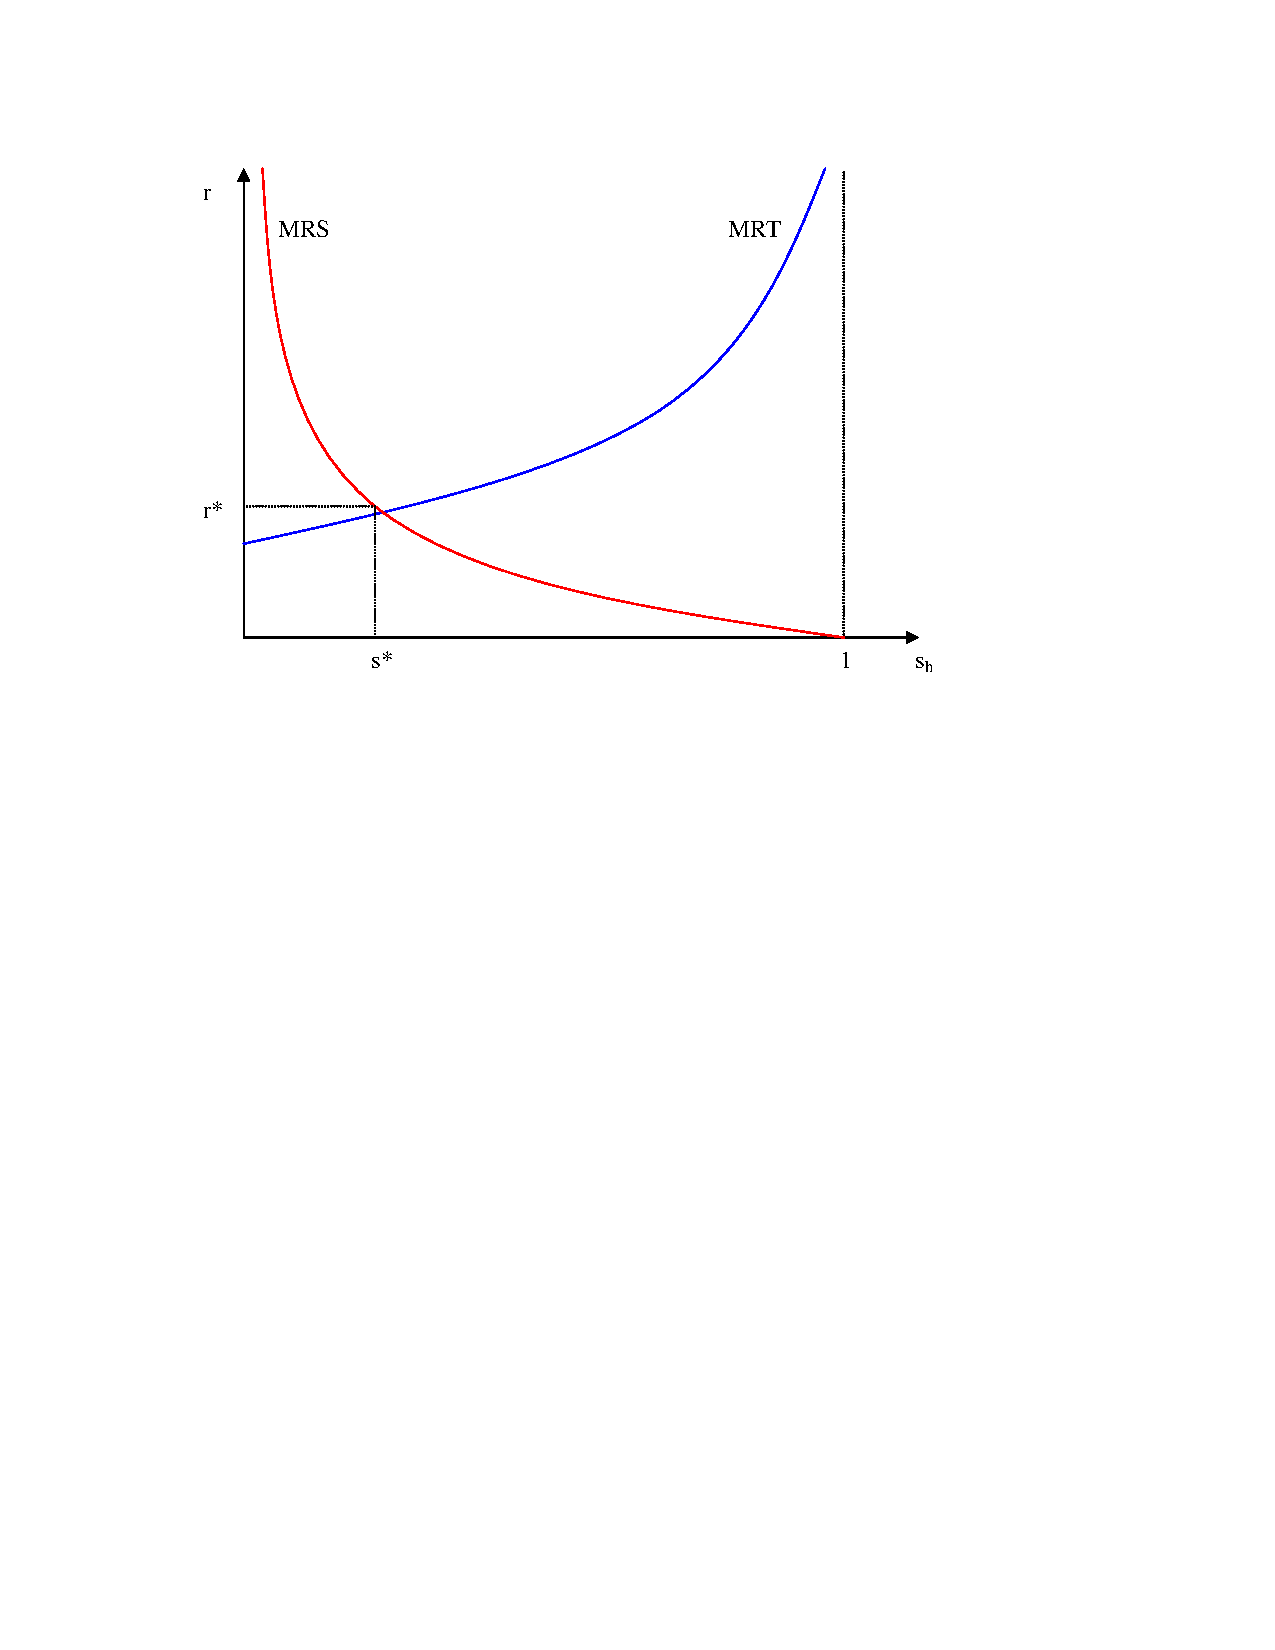
\includegraphics[width=0.7\linewidth]{figures/compstat}\\
  \caption{Residential land and land rents}\label{fig:mrt}
\end{figure}


The equilibrium is characterized by the following condition:
\[
A^\sigma {\lambda}\left[F_L(N/L,1-{\lambda})\right]^\sigma = AF(N/L,1-{\lambda}),
\]
which can then be solved for the equilibrium ${\lambda}$. The LHS is
increasing in $\lambda$, while the RHS is decreasing. Notice how the
equilibrium share of housing depends on the level of development,
$A$. Because $\sigma<1$, the RHS increases faster with development
than the LHS. This implies that the supply of housing, $\lambda$,
increases with development. This crucially depends on consumption
and housing being complements. Development increases the supply of
manufactured goods in proportion to $A$. It also leads to cheaper
manufactured goods, which increases their relative demand. The
increase in demand is smaller, only proportional to $A^\sigma$. The
supply of manufacturing has to adjust downward, the relative supply
of housing adjusts upward.


Because land rents are linear in $A$ for a given $\lambda$, and increase in $\lambda$, we have the following propositions.
\begin{proposition}
Development leads to higher rents, both relative to manufacturing prices and wages. The share of rents in national income and the demand for residential land increase.
\end{proposition}
\begin{proposition}
Land rents increase with population density.
\end{proposition}

\subsection{Two locations}
Now we introduce another location within the country. Both  locations have the same endowment of land but they may differ in their population densities, $N/L$. Without loss of generality, we assume that location 2 has the higher population density, $N_2/L>N_1/L$. We then call this location the ``city,'' the less populous location the ``village.''

The locations interact as follows. Manufacturing goods can be freely transported across locations. People are not allowed to change residence. (We study endogenous urbanization later.) Workers do not commute, so both land and labor are immobile factors.

As before, a lord owns all the land in all locations, and redistributes the rental income for residents in the form of a lump-sum transfer. The budget constraint of the representative household in location $i$ is then
\[
x_i + r_i h_i \le w_i + T.
\]
Total spending on manufactured goods (with a price normalized to one) and rent cannot exceed income from wages and the transfer. The balanced-budget condition of the lord is
\[
TN = r_1L+r_2L.
\]

The equilibrium allocation is such that (i) workers and land are fully employed in both locations, (ii) the global market for manufacturing goods clears, (iii) the local markets for housing clear, (iv) firms maximize profits, and (v) households maximize utility given their budget constraint.

In what follows, we focus on equilibria that feature \emph{complete specialization}, that is, manufacturing only active in one location. It is easy to see that this will be the village and no manufacturing takes place within the city. We will later verify the parameter restrictions that are required for this to be an equilibrium.

In this case, city residents have no wage income, all their income comes from rent transfers. All city land is used for housing, $h_2=L$. The budget constraint of the city is hence
\[
x_2+r_2L = \frac{N_2}{N}(r_1L+r_2L).
\]
Consumption and housing rents have to be covered from transfers that are proportional to total rent in the economy. Letting $\alpha=N_2/N$ denote the fraction of the population that live in the city,
\[
r_2 = \frac{\alpha}{1-\alpha}r_1 -\frac{x_2}{L}.
\]

We construct the equilibrium in the following steps.
\begin{enumerate}
  \item Take a land share of housing ${\lambda}$ in the village. This pins down rent in the village, $r_1$, as the marginal product of land in manufacturing. Clearly, $r_1$ is increasing in ${\lambda}$.
      \[
      r_1 = AF_L(N_1/L,1-{\lambda})
      \]
  \item It also pins down the supply of the manufactured good $x$, because the city has no manufacturing. This supply $x$ is decreasing in ${\lambda}$.
      \[
      \frac{x}{L} = AF(N_1/L,1-{\lambda})
      \]
  \item Given the rent prevailing in the village and the amount of land allocated to housing, we can derive the villagers' demand for manufactured goods, $x_1$. This is increasing in ${\lambda}$, both because of the higher rents, and because of a higher housing consumption.
      \[
      \frac{x_1}{L} = {\lambda}\left[AF_L(N_1/L,1-{\lambda}]\right)^\sigma
      \]
  \item The supply of the manufactured good available to city-dwellers, $x_2=x-x_1$ is hence decreasing in ${\lambda}$.
      \begin{equation}\label{eq:eq1}
      \frac{x_2}{L} = AF(N_1/L,1-{\lambda})-{\lambda}\left[AF_L(N_1/L,1-{\lambda})\right]^\sigma
      \end{equation}
  \item The demand for manufactured goods in the city is pinned down by the city rent, $r_2$:
      \begin{equation}\label{eq:eq2}
      \frac{x_2}{L} = r_2^\sigma.
      \end{equation}
  \item There is also the budget constraint of the city,
  \begin{equation}\label{eq:eq3}
    \frac{x_2}{L} = \alpha r_1 -(1-\alpha)r_2 = \alpha \left[AF_L(N_1/L,1-{\lambda})\right]^\sigma -(1-\alpha)r_2.
  \end{equation}
\end{enumerate}
Equations \eqref{eq:eq1}, \eqref{eq:eq2} and \eqref{eq:eq3} can be solved for ${\lambda}$, $r_2$ and $x_2$. We combine \eqref{eq:eq2} and \eqref{eq:eq3} to substitute out $r_2$. This leads to an equation that gives the \emph{demand} for $x_2$ as a function of $\lambda$. Higher $\lambda$ implies higher land rents in the village, part of which increases the income of city residents, leading to higher city demand for the manufactured good. Equation \eqref{eq:eq1} then characterizes the \emph{supply} of $x_2$. Higher $\lambda$ implies lower manufacturing production and a lower supply of $x_2$.

These demand and supply schedules are plotted on Figure \ref{fig:stage2}. We conduct two comparative statics. First, we increase $A$ to capture technical progress. Note that this increases both the demand and the supply of $x_2$, but the supply more than the demand, so the manufactured good has to become cheaper. Second, we increase $\alpha$, the fraction of people living in the city. In the current setup, because there is no production in the city, this only constitutes a larger income transfer from the village to the city.

\begin{figure}[h!]
\centering
  % Requires \usepackage{graphicx}
  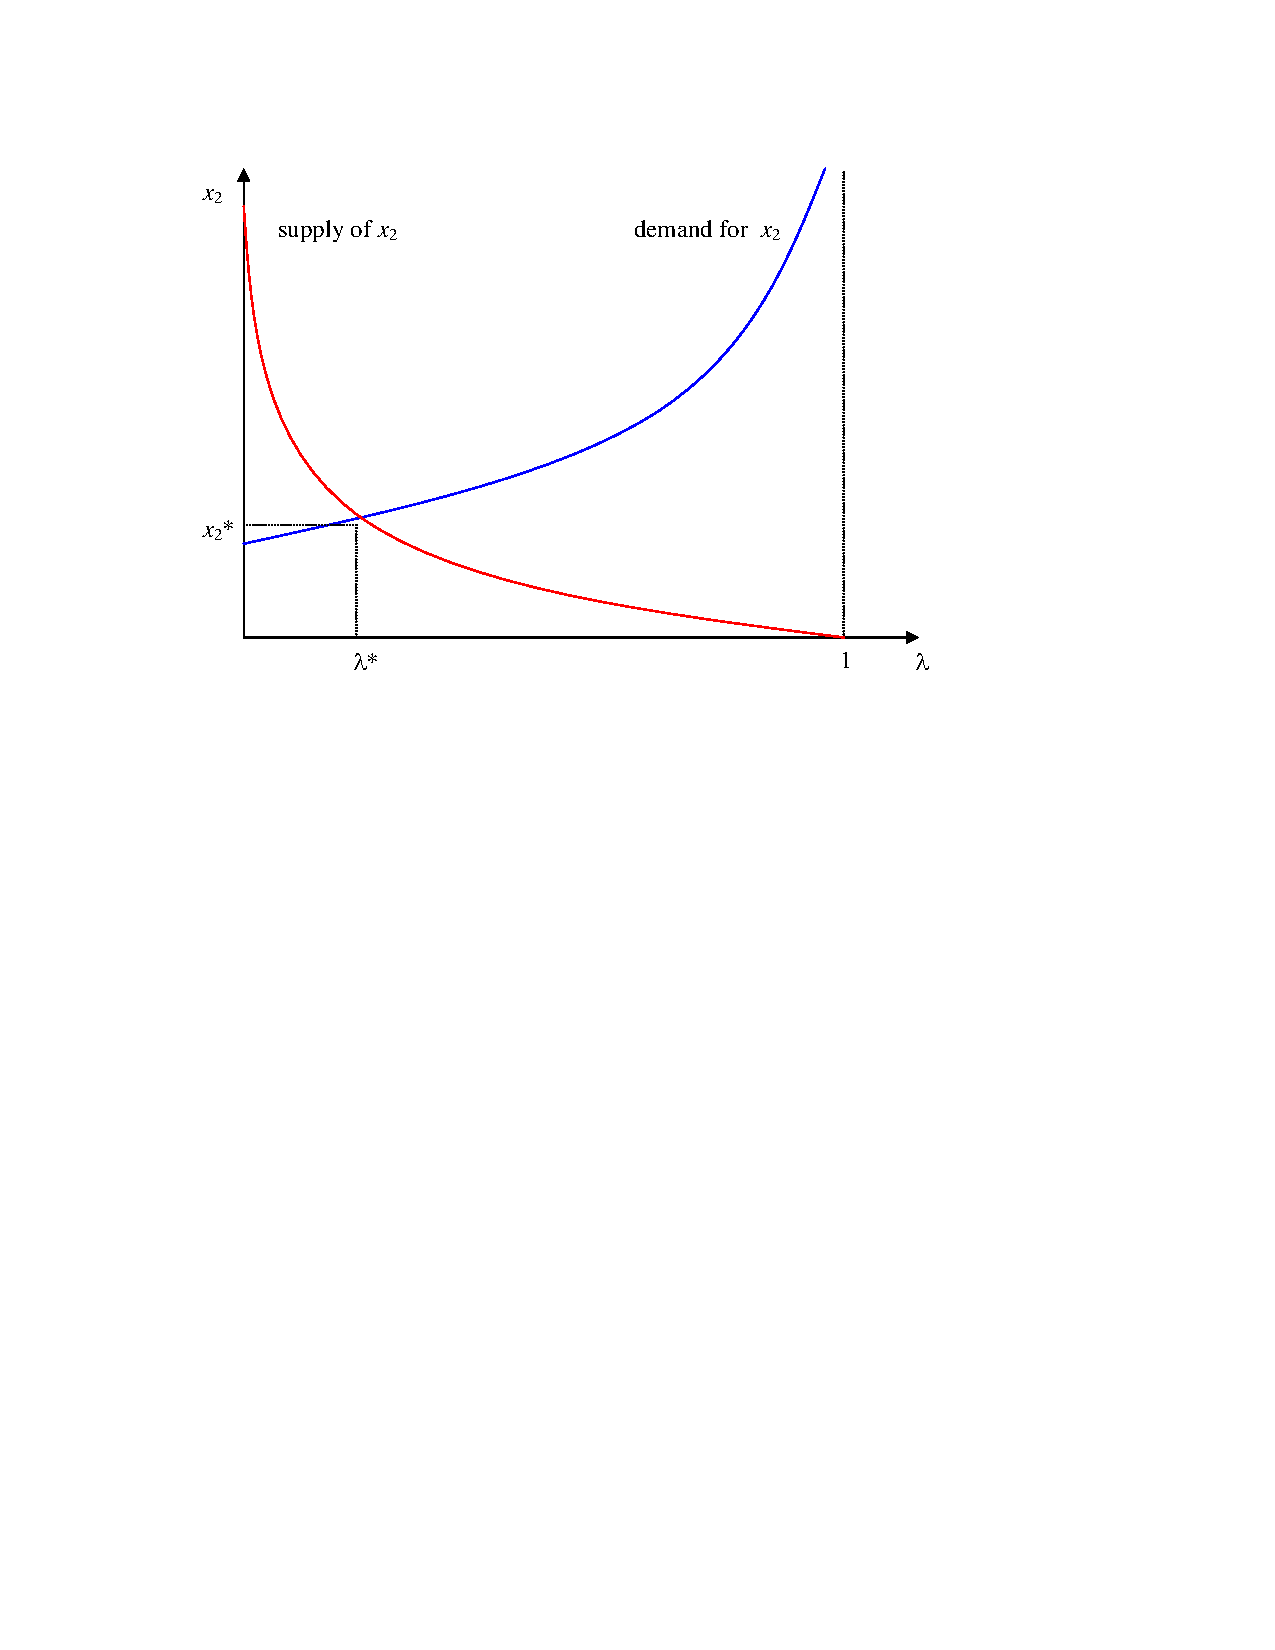
\includegraphics[width=0.7\linewidth]{figures/compstat2}\\
  \caption{The demand and supply of manufactured goods in the city}\label{fig:stage2}
\end{figure}


\begin{proposition}
City rents increase faster with development than village rents.
\end{proposition}
The intuition for this result is that because rents increase faster than manufacturing TFP, rental income will outpace wage income. Since city residents earn a larger fraction of the rental income, this constitutes a transfer from the village to the city. Such a transfer raises the price of city housing relative to village housing.

\begin{proposition}
Urbanization leads to higher manufacturing output, lower village rents, and higher city rents.
\end{proposition}
Because urbanization (for a given population density in the village, $N_1/L$) only entails a transfer of rents, the supply schedule of manufacturing goods is unaffected, whereas the demand schedule shifts up. This leads to lower village housing (hence lower rents) and higher manufacturing output. The high manufacturing consumption in the city can only be sustained with higher city rents.


\subsection{Introducing services}
We introduce services in the simplest way. The final good $x$ is broken up as a Cobb-Douglas composite of manufacturing and services,
\[
x = m^\gamma s^{1-\gamma},
\]
so that total utility is
\[
u(m,s,h) = \left[\left(m^{\gamma}s^{1-\gamma}\right)^{1-1/\sigma}+h^{1-1/\sigma}\right]^{\sigma/(\sigma-1)}.
\]

Both manufacturing and services are produced using the same technology
\begin{align*}
m&=AF(n_m,l_m),\\
s&=AF(n_s,l_s),
\end{align*}
and will hence have the same price in a location in which both are produced. We make this assumption to emphasize that none of our results are driven by technological differences. The only difference between manufacturing and services is that while manufactured goods can be freely traded across locations, services have to be consumed in the location in which they were produced.

The budget constraint of the representative household in location $i$ is
\[
m_i + p_is_i + r_i h_i \le w_i + T,
\]
where $p_i$ is the price of services in location $i$. Note that this is unity if the manufacturing good is produced in location $i$ (because the two industries have the same cost functions), however, it may be greater than 1 if the manufacturing sector is inactive.

The equilibrium allocation is such that (i) workers and land are fully employed in both locations, (ii) the global market for manufacturing goods clears, (iii) the local markets for services and housing clear, (iv) firms maximize profits, and (v) households maximize utility given their budget constraint.

Again, we focus on complete specialization equilibria. In these equilibria, manufacturing only produces in the village, which pins down services prices in the village as $p_1=1$. Service prices in the city are higher, $p_2>1$.

When constructing the equilibrium, we first observe that, in the village, both services and manufacturing use the same factor proportions. This is implied by the profit maximization of firms that face common wages, rents, and technologies. If ${\lambda_1}$ share of land is allocated to housing in the village, then the total land used in production is $(1-{\lambda_1})L$. The ratio of workers to land in both industries is
\[
\frac{n_{m1}}{l_{m1}}=\frac{n_{s1}}{l_{s1}}=\frac{N_1}{(1-{\lambda_1})L}.
\]
The marginal product of land only depends on the factor proportions so it continues to be
\[
r_1 = AF_L(N_1/L,1-{\lambda_1}),
\]
just as in the case without services. Also, because of the identical technologies, we can simply write the total supply of manufacturing and services in the village as
\[
y_{m}+s_1 = ALF(N_1/L,1-{\lambda_1}),
\]
where $y_{m}$ is the village supply of manufacturing (which may be different from the village demand).

The total expenditure on services and manufacturing depends on the rent,
\[
\frac{m_1+s_1}{h_1}  = r_1^\sigma.
\]
The excess supply (net exports) of manufacturing is supply minus demand, $y_m-m_1$. This is simply
\begin{equation}\label{eq:eq1b}
\frac{y_m-m_1}{L} = \frac{(y_m+s_1)-(m_1+s_1)}{L} = AF(N_1/L,1-{\lambda_1}) - \lambda_1\left[AF_L(N_1/L,1-{\lambda_1})\right]^\sigma,
\end{equation}
the same as in the previous case, \eqref{eq:eq1}.

The budget constraint of the city is
\[
m_2 +p_2s_2+r_2h_2 = w_2N_2+TN_2.
\]
Spending on manufactures, services and housing equal the wage income plus transfers. Because the service technology is CRS, services firms make zero profit:
\[
p_2s_2 = w_2N_2+r_2(L-h_2).
\]
The total income of the service sector in the city equals the sum of the total city wagebill and the rents paid on land used by services. The budget constraint can then be rewritten as
\[
m_2 +r_2L = TN_2,
\]
which is again the same as before. (Spending on manufactures and the total land rent in the city equals the transfer income.) Writing out transfers,
\begin{equation}\label{eq:eq3b}
    \frac{m_2}{L} = \alpha r_1-(1-\alpha)r_2 = \alpha \left[AF_L(N_1/L,1-{\lambda_1})\right]^\sigma-(1-\alpha)r_2.
\end{equation}
This equation is identical to \eqref{eq:eq3}. Both the supply of manufactured goods available in the city and the budget constraint of city residents is identical to the previous case.  %This is what we turn next.

As in the previous setup, city rents increase faster than both village rents and village wages. This translates into relative price differentials, just as predicted by Balassa and Samuelson.
\begin{proposition}
Development raises the relative price of services in the city.
\end{proposition}
We also have the following conjecture.
\begin{conjecture}
The impact of development on service prices is stronger in more urban economies, where a bigger fraction of people live in cities.
\end{conjecture}
This statement holds true in the two extremes: if the two locations are of equal size, there is no specialization, and service prices will always equal manufacturing prices. With high-enough urbanization, there is complete specialization, which implies a positive impact of development on the relative price of services to manufacturing. We conjecture that this holds for intermediate degrees of urbanization, as well.


\section{Empirical results}\label{empirics}
In this section, we present some suggestive evidence supporting the
main mechanisms of the model.

\subsection{Urbanization and prices}
Figure \ref{fig:penn_joint} shows the well known result that higher
per capita income is related to higher aggregate price level. We also show that
higher urbanization increases this influence of per capita income on
the price level and has a similar effect of the relative
non-tradable/tradable prices in standard cross-country regressions.

\begin{figure}[h!]
\centering
  % Requires \usepackage{graphicx}
  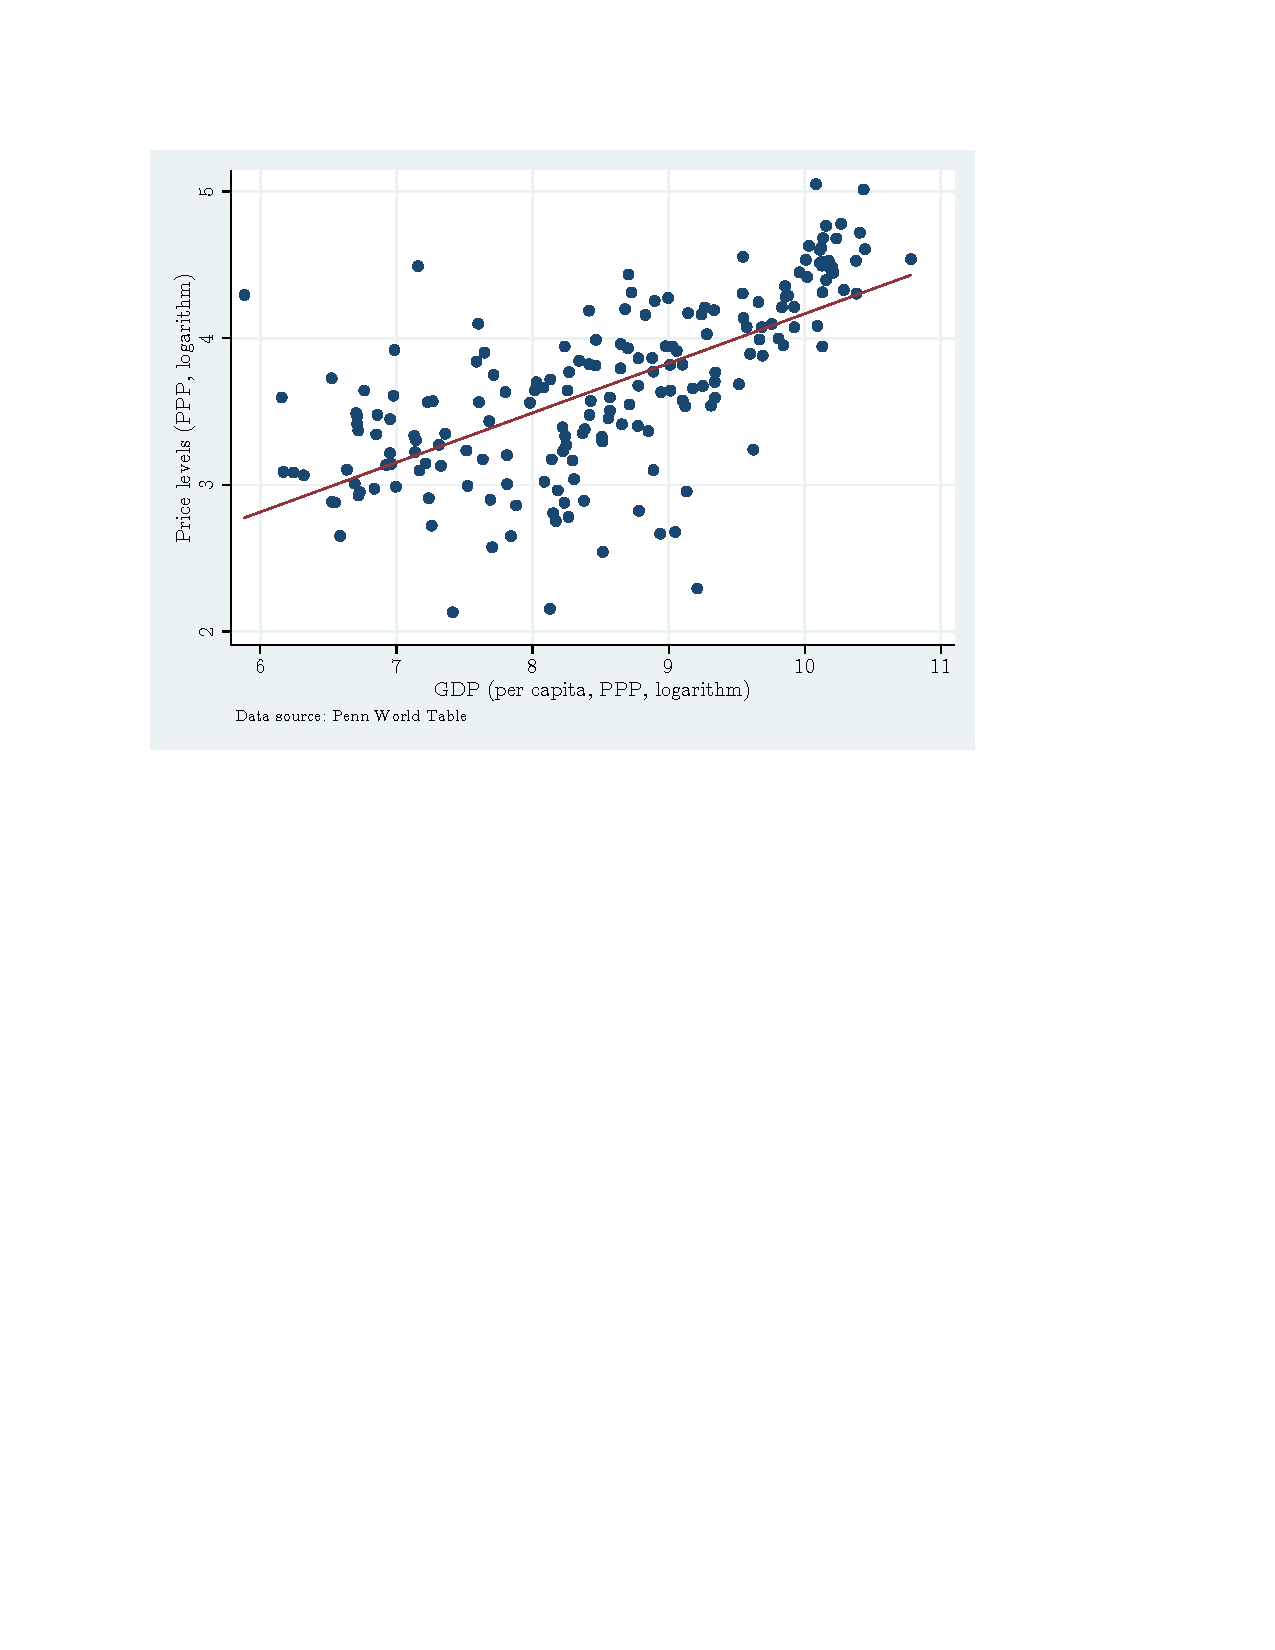
\includegraphics[width=0.7\linewidth]{figures/sc_penn_joint}\\
  \caption{Price levels and per capita GDP across countries}\label{fig:penn_joint}
\end{figure}

Two related, but distinct measures we can use to compare the
urbanization level of a country are the proportion of urban
population and the population density, both available for a large
number of countries from the World Development Indicators database.
As our main question is the difference in the 'closeness of
residents', both measures are imperfect,\footnote{Population
weighted population-density would be a measure which would express
the best the scarcity of land in a country. We are about to develop
this measure using the detailed population and land area measures of
the LandScan database.} but we consider the proportion of urban
population a better measure, as it can be expected to capture the
clustering of the population better than just the average population
density in a country. As the the definition of urban population is
different in every country, however, the cross-country results
should be treated with some caution.

Using the proportion of urban population to divide the sample
equally to more rural and more urbanized countries, Figure
\ref{fig:pennX} shows the cross-country relationships of the (log) price levels
and the (log) per capita GDP for both groups, using data from the
Penn World Table. The graphs shows, in line with our conjecture,
that the relationship between income and the price level is stronger
among more urbanized countries. It also shows that the comparison is
valid as there are reasonable variation in per capita GDP for both
groups, even if there are clearly more high-income countries among
the more urbanized ones.

\begin{figure}[h!]
\centering
  % Requires \usepackage{graphicx}
  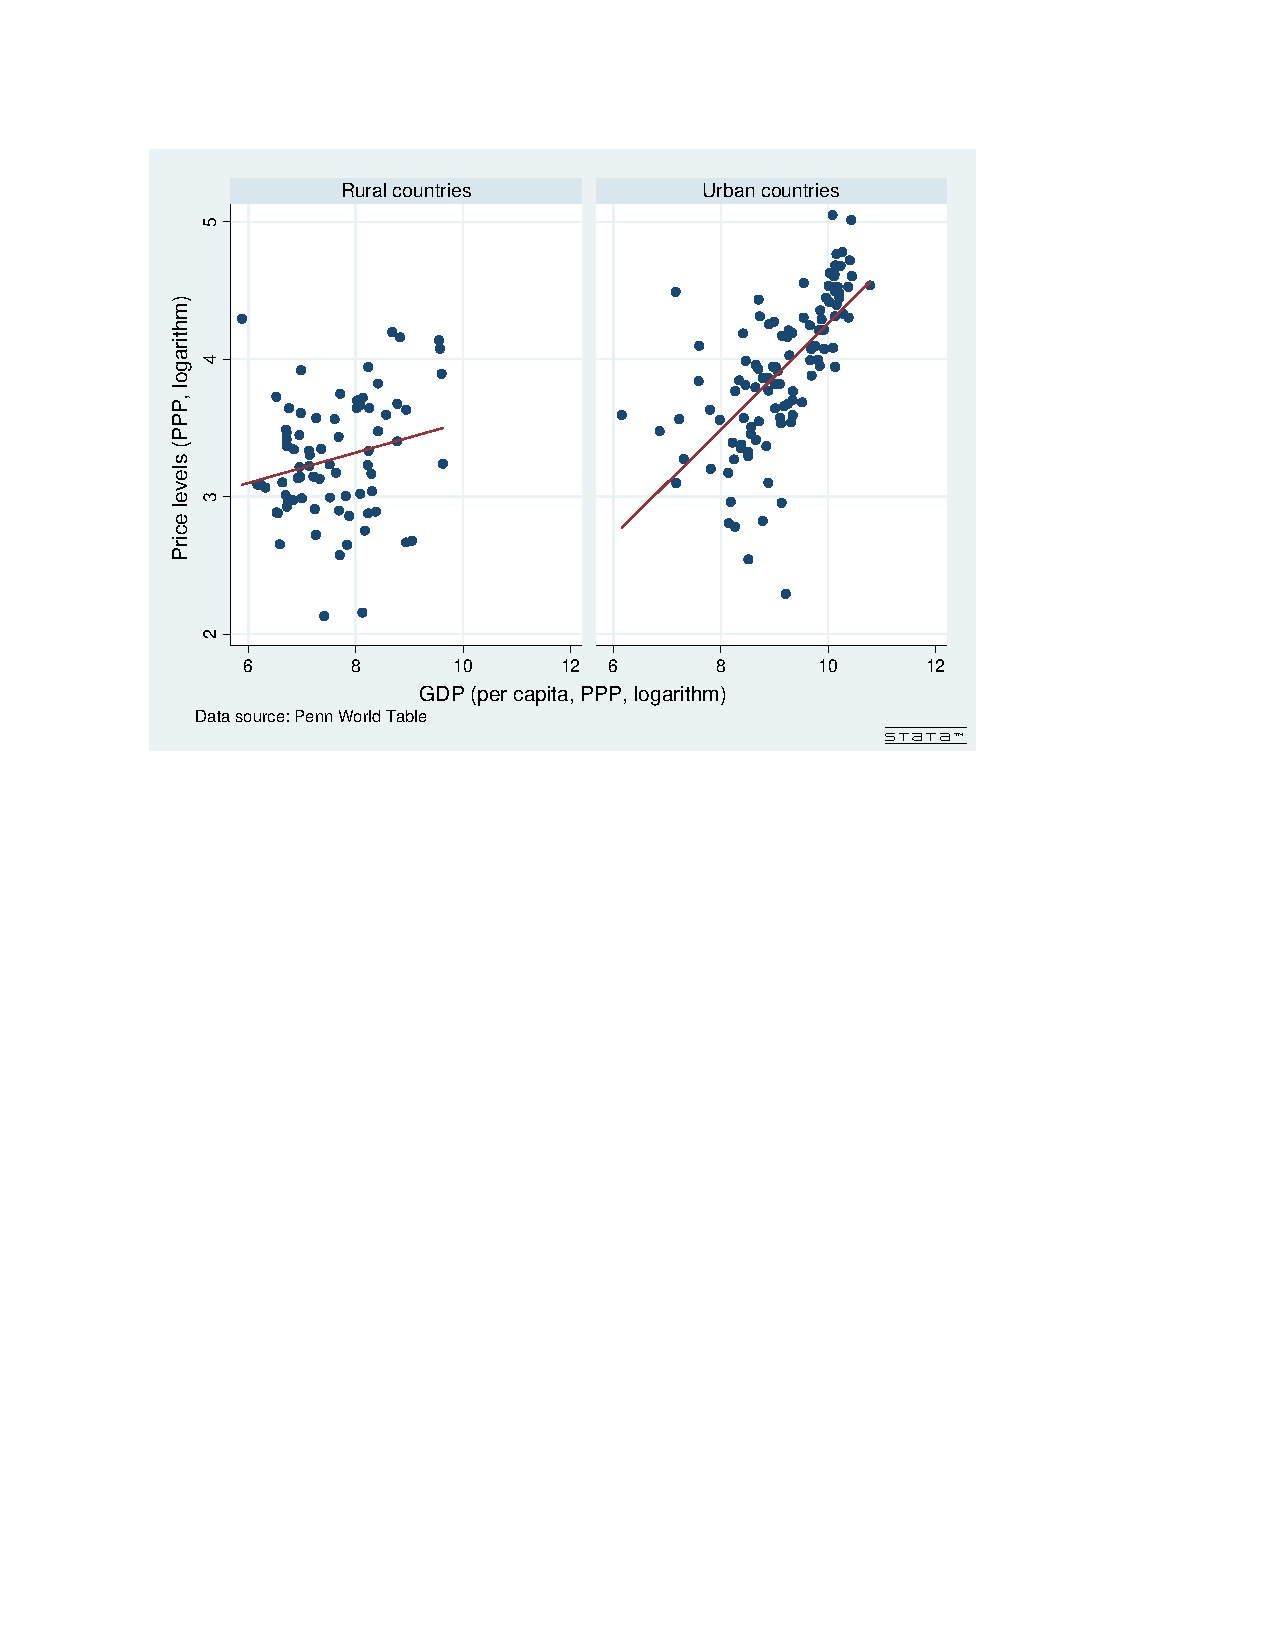
\includegraphics[width=0.7\linewidth]{figures/sc_penn}\\
  \caption{Development, urbanization, and price levels}\label{fig:pennX}
\end{figure}


To approach the question more formally, we estimated some
regressions in the following form
\begin{equation}
\log{P}=\alpha_1+\alpha_2\log Y+\alpha_3Z+\alpha_4(Z-\bar{Z})(\log Y-\overline{\log Y})+\varepsilon,
\end{equation}
where $P$ refers to the various price measures, Y is the measure of
GDP, and $Z$-s are the different urbanization measures. Our main
interest is in the (demeaned) cross-term, as it can be expected to
capture how the level of urbanization influences the relationship
between the output and the price measures.

Our main price measure is the comparable price level available for
over 180 countries from the Penn World Table.\footnote{The sample
extends the 115 benchmark countries, that directly participated the
1996 round of the International Comparison Project(ICP), by using
somewhat less reliable price data and other observable variables.
Our results are robust to restricting the sample to the benchmark
countries.} To check the robustness of the results, we also
calculated a non-tradable/tradable relative price index
($P_{NT}/P_{T}$) using the basic heading level price data for
consumption for the 1996 benchmark ICP countries. This relative
price is more in line with the Balassa-Samuelson proposition
implying that the main reason of the price level difference is the
relatively more expensive non-tradable prices. The measure, however,
can be expected to be less reliable than the aggregate price level
as the non-tradable prices, like services, tend to be less
comparable internationally than tradable prices,

\begin{table}[h!]
\caption{Balassa-Samuelson regressions with urbanization (Robust
standard errors are in parentheses)} \center \label{tab:BS}
\begin{tabular}{c|cc|cc}
  \hline\hline
  Explanatory & \multicolumn{4}{c}{Dependent variables} \\
  variables &\multicolumn{2}{c}{$\log P$} & \multicolumn{2}{c}{$\log(P_{NT}/P_T)$} \\ \hline
  $\log Y$ & \textbf{0.25} & \textbf{0.34} & \textbf{0.28}   & \textbf{0.33} \\
           & (0.05)        & (0.03)        & (0.07)          & (0.05)        \\
  urban    & \textbf{0.61} &               & 0.12            &               \\
           & (0.21)        &               & (0.34)          &               \\
  urbanX   & \textbf{0.38} &               & \textbf{0.43}   &              \\
           & (0.11)        &               & (0.19)          &              \\
  log(density) &           & -0.02         &                 & -0.02        \\
             &             & (0.02)        &                 &  0.04        \\
  densityX &               & \textbf{0.05} &                  & 0.01         \\
           &               & (0.02)        &                 & 0.02         \\
  constant & \textbf{1.13} & \textbf{0.82} & \textbf{-2.96}  & \textbf{-3.13}\\
           & (0.31)        & (0.26)        & 0.50            & (0.41)        \\ \hline
  No. of obs. & 186        & 183           & 113             & 113          \\
  $R^2$    & 0.50          & 0.46          & 0.38            & 0.34  \\
  \hline\hline
\end{tabular}
\end{table}

Table \ref{tab:BS} implies that the regressions mostly support our
conjectures. The first two columns use the (log) price levels as
dependent variables, while the last two uses the (log) relative
non-tradable/tradable prices. For both dependent variables, we
present two regressions with the two urbanization measures. 'Urban'
is the proportion of urban population, and 'density' is the
population density; and 'urbanX' and 'densityX' are the demeaned
output-urbanization cross terms.

In line with well known previous results, higher per capita output
increases both the price level and the relative prices across
countries, but this relationship is significantly influenced by the
level of urbanization, even after controlling for direct price
effects of the urbanization. Looking at the first regression, we
have found that 1 percent higher per capita output increases the price
level by 0.25 percent for average level of urbanization (54 percent), and 1 percent
higher urbanization has a further 0.61 percent direct effect. The cross
effect, however, implies that the effect of output on the prices
would be close to 0 under the (extreme) case of 0 urbanization
($0.25-0.54\cdot0.38=0.05$) and would be over 0.4 in case of full
urbanization. The effects using the relative prices are similar
supporting the conjecture that the price differences are the result
of different non-tradable prices. Using the population density as
explanatory variable still supports the effect using the price
level, though it turns out to be insignificant for our sample in
explaining the cross country relative price differences.

\subsection{Industry location}
An important starting point of the model is the assumption that
non-tradables have to be produced close to the consumers. An
implication of this spatial assumption is that higher urbanization
of the population in an area would imply higher relative employment
in the non-tradable sectors than in the tradeable ones. We have
examined this mechanism by looking at the US Census 2000
data.\footnote{The more detailed survey covering approximately 15 percent
of the households contains detailed (NAICS 2 digit level)
information about the industry level employment, while the general
short survey contains information about the urban population and
population density according to various geographic areas}

Figure \ref{fig:nt-states} shows the relationship between the proportion of urban
population and the relative non-tradable/tradable employment for US
states, strongly supporting the conjectured positive relationship.

\begin{figure}[h!]
\centering
  % Requires \usepackage{graphicx}
  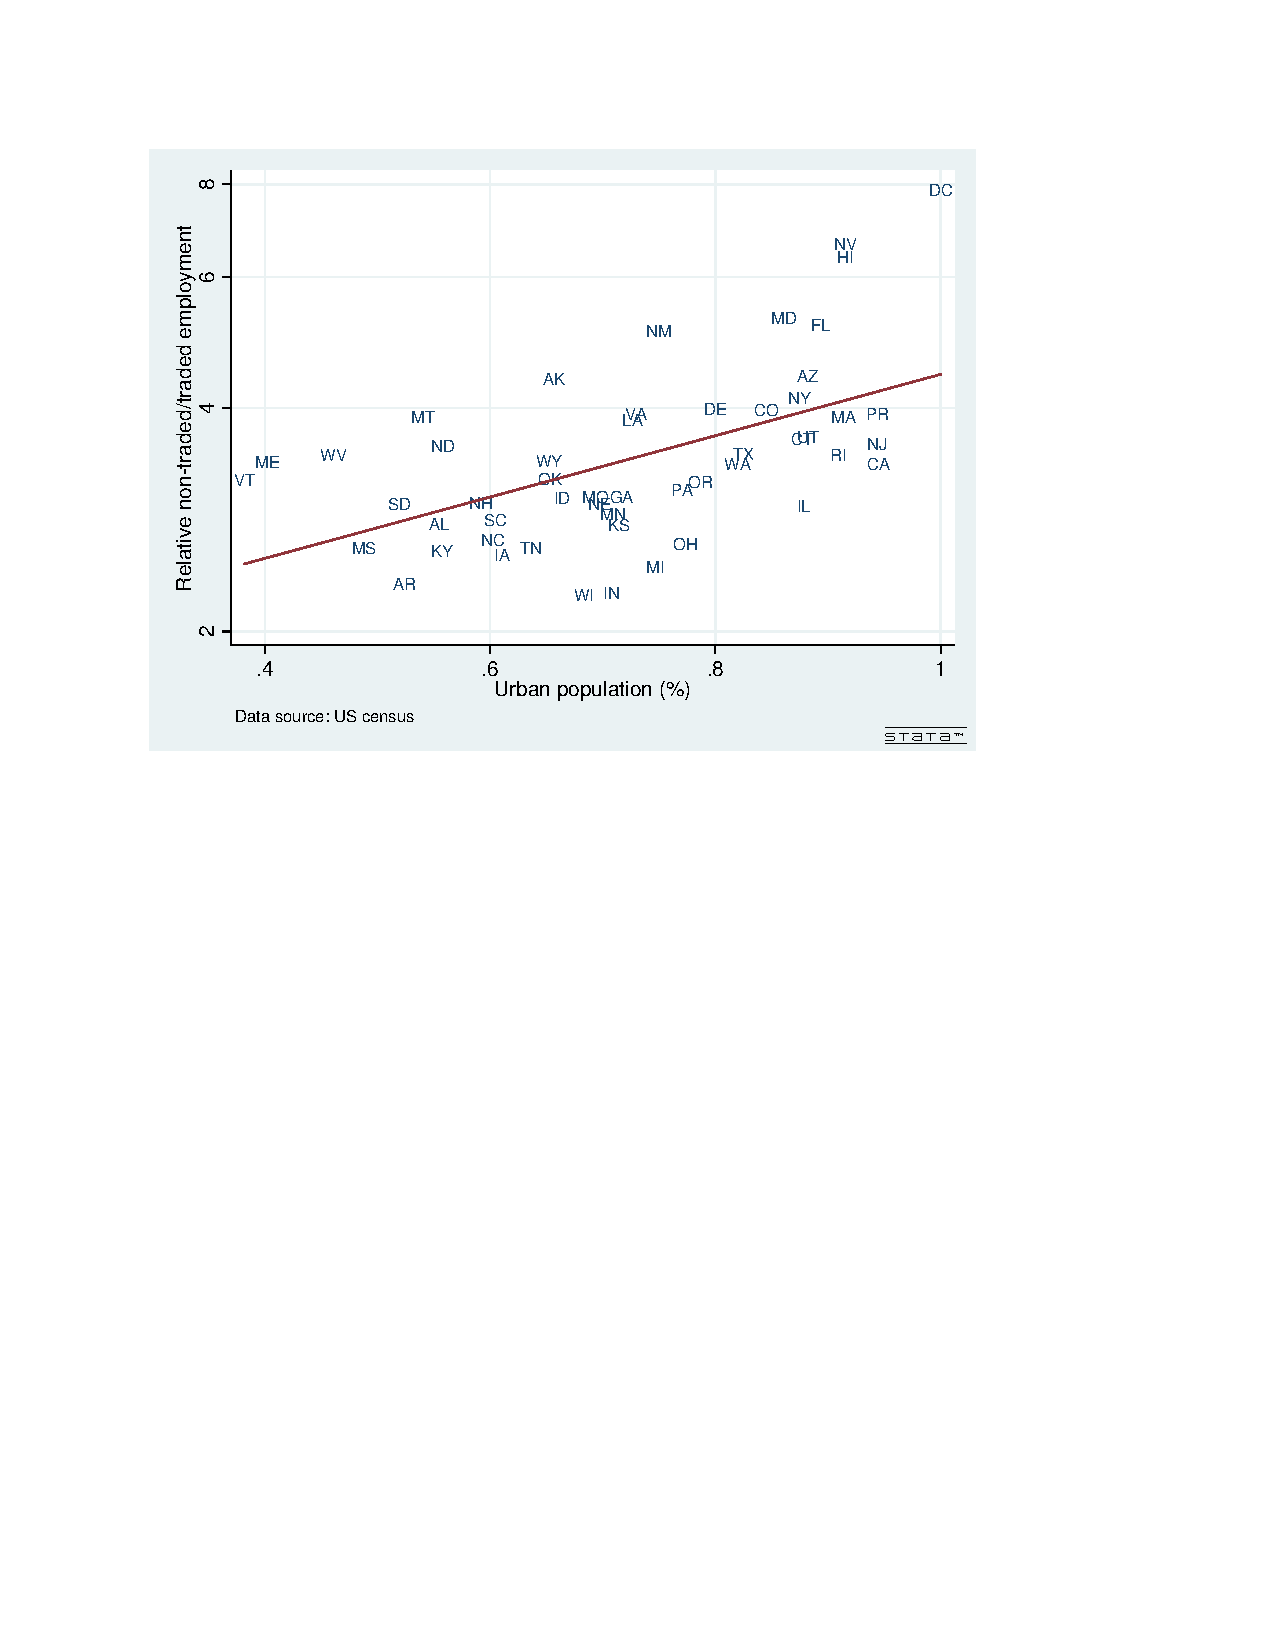
\includegraphics[width=0.7\linewidth]{figures/sc_state}\\
  \caption{Urbanization and non-traded employment in U.S.~states}\label{fig:nt-states}
\end{figure}


To examine the effects more formally, we used US county level data.
The advantage of using counties is that it can capture the
population clustering better than state level data and covers the
whole country, though a potential problem is that if a large number
of the employees live and work in different
counties.\footnote{Metropolitan statistical areas are a possible
alternatives taking commuting habits into consideration, but,
naturally, do not covering the whole country. Our regressions are
robust to using these areas as well.} As before, we used the
proportion of urban population and population density as measures of
urbanization and also included the (log) per capita median income
within the county.

\begin{table}[h!]
\center \caption{Urbanization and relative NT/T employment (Robust
standard errors are in parentheses)}
\begin{tabular}{c|cc}
  \hline\hline
  Explanatory & \multicolumn{2}{c}{Dependent variable} \\
  variables & \multicolumn{2}{c}{$\log (N_{NT}/N_T)$} \\ \hline
  urban         & \textbf{0.62} &  \\
                & (0.02)        &  \\
  log(density)  &               & \textbf{0.07} \\
                &               & (0.01) \\
  log(income)   & \textbf{0.11} & \textbf{0.18} \\
                & (0.02)        & (0.03) \\
  constant      & -0.53         & \textbf{-1.18} \\
                & (0.28)        & (0.30) \\ \hline
  $R^2$         & 0.20          & 0.10 \\
  No. of obs.   & 3218          & 3218 \\ \hline\hline
\end{tabular}
\end{table}

The results show that even after correcting for the median income,
the level of urbanization -- measured in the proportion of urban
population or population density -- significantly increases the
proportion of employees working in non-tradable sectors supporting
our spatial correlation assumption.

\subsection{Land prices and income}
The effects of development on the price of land is a major mechanism
in our model influencing the relative price of services. To have a
first look at the question, we use the dataset constructed by Davis and
Palumbo (2008) who created implied residential land value data for 46
large U.S.~metropolitan areas. To get this data, the authors use
regional data on construction costs and decompose the value of an
average home to replacement value and land value.

\begin{figure}[h!]
\centering
  % Requires \usepackage{graphicx}
  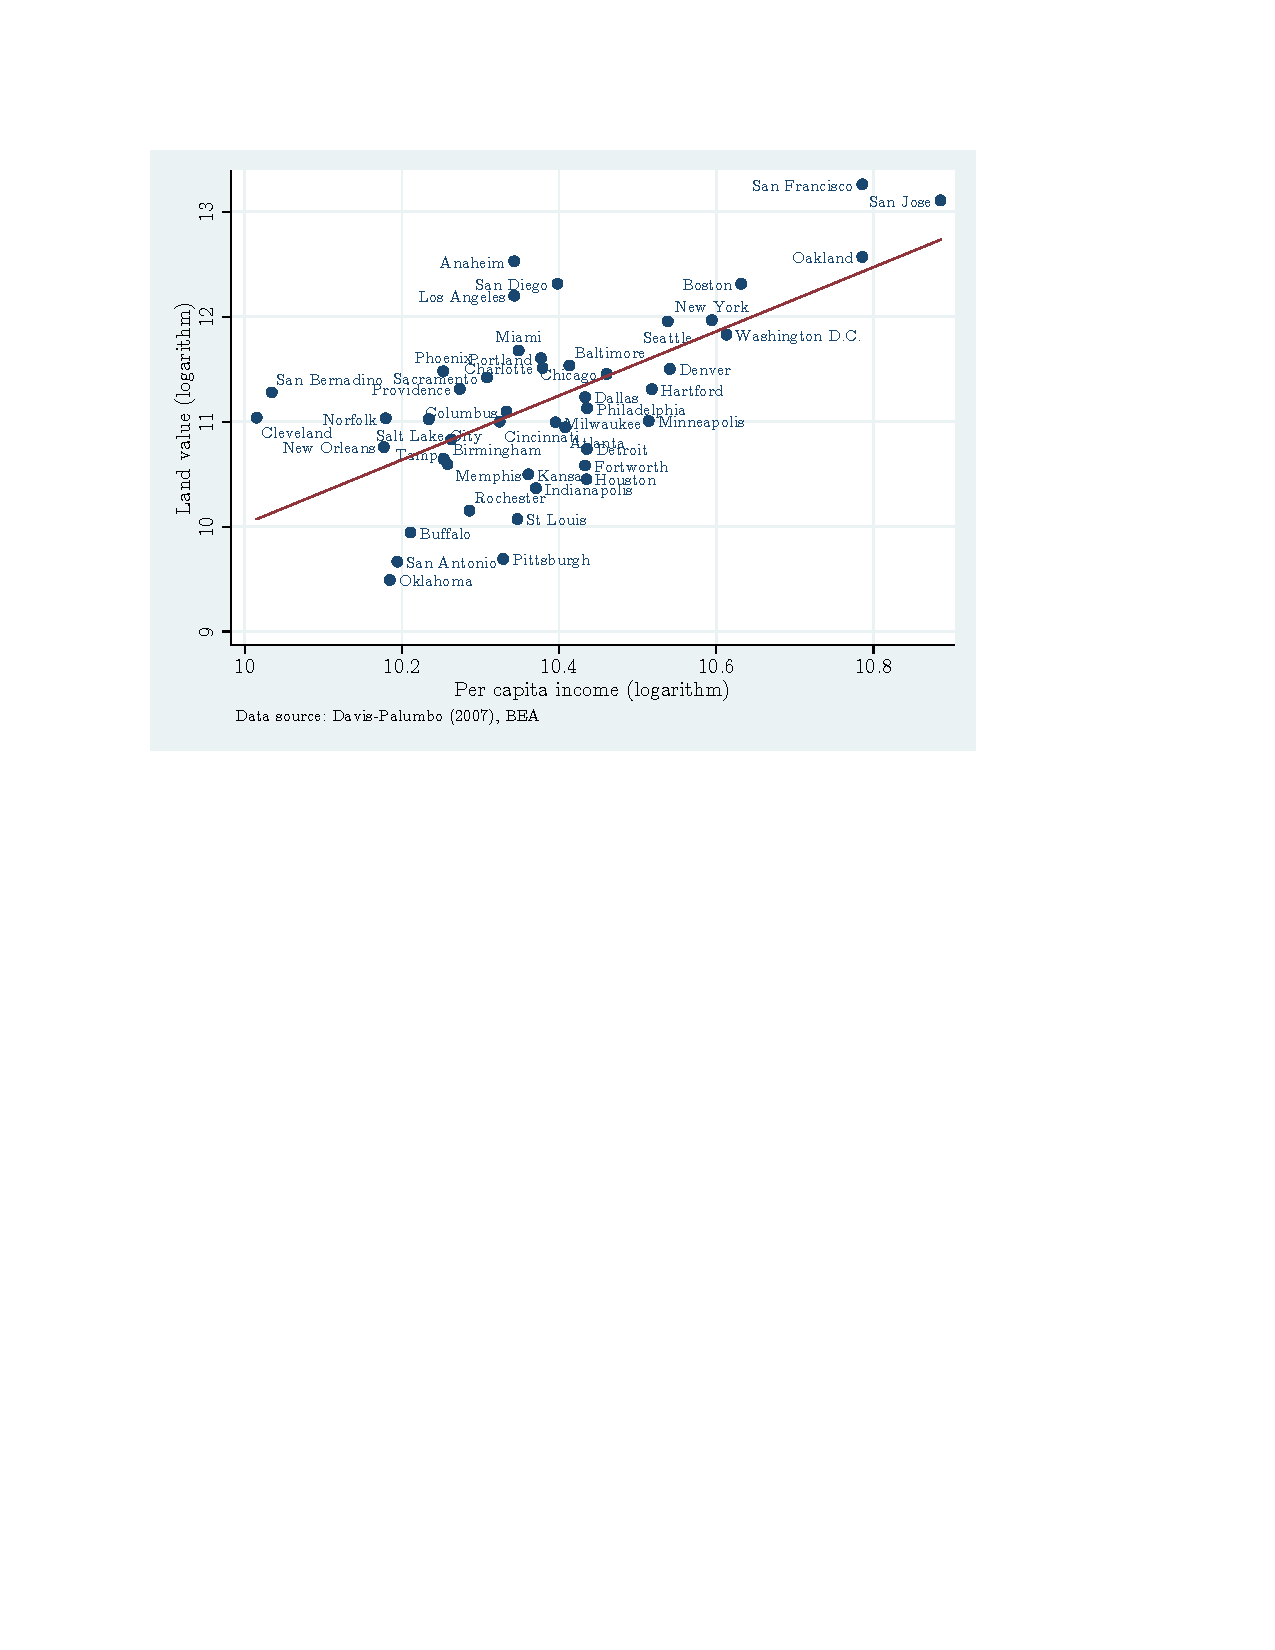
\includegraphics[width=0.7\linewidth]{figures/sc_davis}\\
  \caption{Land prices and income across large US cities}\label{fig:land}
\end{figure}

Figure \ref{fig:land} shows the (log) price of land as a function of
per capita income for the U.S.~cities. It strongly supports our
conjecture that higher income areas face more appreciated land
prices.

Table \ref{tab:land} shows the estimated effects of income on the
land prices, the replacement values (constr) and home values
controlling for the size of the metropolitan areas. The regressions
show that the regional income influences all the values, but it has
the largest effect on the land prices with an amplification factor
of 2.8. This is consistent with our model, in which the complementarity between land and consumption leads to an amplified response of rents to income.

\begin{table}[h!]
\center \caption{Land prices and income (Robust standard errors are
in parentheses)} \label{tab:land}
\begin{tabular}{c|ccc}
  \hline\hline
  Explanatory & \multicolumn{3}{c}{Dependent variable} \\
  variables & log(land) & log(constr) & log(home) \\ \hline
  log(income)    & \textbf{2.77}   & \textbf{0.38}  & \textbf{1.66}\\
                 & (0.67)          & (0.11)         &  (0.38)\\
  log(population)& 0.13            &  0.02          &  0.05\\
                 & (0.18)          & (0.03)         &  0.10\\
  constant       & \textbf{-19.47} & \textbf{7.38}  &  -5.83\\
                 & (6.35)          & (1.12)         &  (3.53)\\ \hline
  $R^2$          & 0.42            & 0.25           &   0.52\\
  No. of obs.    & 46              & 46             &   46   \\ \hline\hline
\end{tabular}
\end{table}

\section{Conclusion}
[TO BE WRITTEN]

\begin{thebibliography}{99}
\bibitem{Balassa64} Balassa, B., 1964, ``The Purchasing-Power Parity Doctrine: A
Reappraisal,'' \emph{Journal of Political Economy}, 584-596.
\bibitem{Davis07} Davis, M. A. and Heathcote, J., 2007, ``The Price and Quantity of Residential Land in the United States,'' \emph{Journal of Monetary Economics} 54:2595-2620.
\bibitem{Davis07} Davis, M. A. and Palumbo, M. G., 2008, ``The Price
of Residential Land in Large U.S. Cities,'' \emph{Journal of Urban Economics}, 63:352--384.
\bibitem{} Davis, M. A. and Ortalo-Magne, F., 2007, ``Household Expenditures, Wages, Rents,'' working paper.
\bibitem{Heston06} Heston, A., R. Summers and B. Aten, 2006, Penn World Table Version 6.2, \emph{Center for International Comparisons of Production, Income and Prices at the University of
Pennsylvania}
\bibitem{Klenow07} Hsieh, C.T and Klenow, P.J, ``Relative Prices and
Relative Prosperity,'' \emph{The American Economic Review}, 562-585.
    \bibitem{Obstfeld99} Obstfeld, M. and Rogoff, K., 1996, \emph{Foundations of International
Macroeconomics}, The MIT Press, Cambridge MA
    \bibitem{Samuelson64} Samuelson, P. A. , 1964, ``Theoretical Notes on Trade
Problems,'' \emph{The Review of Economics and Statistics}, 145-154.
    \bibitem{} Tang, X., 2007, ``The Rich Neighborhood Effect versus the Balassa-Samuelson Effect: An Income-Based Explanation of International Price Level Differences,'' working paper.
\end{thebibliography}

\end{document}
